% mnras_template.tex 
%
% LaTeX template for creating an MNRAS paper
%
% v3.0 released 14 May 2015
% (version numbers match those of mnras.cls)
%
% Copyright (C) Royal Astronomical Society 2015
% Authors:
% Keith T. Smith (Royal Astronomical Society)

% Change log
%
% v3.0 May 2015
%    Renamed to match the new package name
%    Version number matches mnras.cls
%    A few minor tweaks to wording
% v1.0 September 2013
%    Beta testing only - never publicly released
%    First version: a simple (ish) template for creating an MNRAS paper

%%%%%%%%%%%%%%%%%%%%%%%%%%%%%%%%%%%%%%%%%%%%%%%%%%
% Basic setup. Most papers should leave these options alone.
\documentclass[fleqn,usenatbib]{mnras}

% MNRAS is set in Times font. If you don't have this installed (most LaTeX
% installations will be fine) or prefer the old Computer Modern fonts, comment
% out the following line
\usepackage{newtxtext,newtxmath}
% Depending on your LaTeX fonts installation, you might get better results with one of these:
%\usepackage{mathptmx}
%\usepackage{txfonts}

% Use vector fonts, so it zooms properly in on-screen viewing software
% Don't change these lines unless you know what you are doing
\usepackage[T1]{fontenc}

% Allow "Thomas van Noord" and "Simon de Laguarde" and alike to be sorted by "N" and "L" etc. in the bibliography.
% Write the name in the bibliography as "\VAN{Noord}{Van}{van} Noord, Thomas"
\DeclareRobustCommand{\VAN}[3]{#2}
\let\VANthebibliography\thebibliography
\def\thebibliography{\DeclareRobustCommand{\VAN}[3]{##3}\VANthebibliography}


%%%%% AUTHORS - PLACE YOUR OWN PACKAGES HERE %%%%%

% Only include extra packages if you really need them. Common packages are:
\usepackage{graphicx}	% Including figure files
\usepackage{amsmath}	% Advanced maths commands
\usepackage{siunitx}    % units for physical quantities
\usepackage{hyperref}   % links to github
% \usepackage[frozencache,cachedir=.]{minted}  % code block in appendix
% \usepackage{minted}
\usepackage{multirow, makecell}   % used to place images in tensions table
\usepackage[table]{xcolor}     % coloured rows in table
\usepackage{color, soul}% Highlighting todo
% \usepackage{amssymb}	% Extra maths symbols

%%%%%%%%%%%%%%%%%%%%%%%%%%%%%%%%%%%%%%%%%%%%%%%%%%

%%%%% AUTHORS - PLACE YOUR OWN COMMANDS HERE %%%%%
\newcommand{\ncr}[2]{{}^{#1}C_{#2}}
\newcommand{\lcdm}{$\Lambda$CDM}
\newcommand{\dmb}{\ensuremath{\Delta m_\mathrm B}}

% Please keep new commands to a minimum, and use \newcommand not \def to avoid
% overwriting existing commands. Example:
%\newcommand{\pcm}{\,cm$^{-2}$}	% per cm-squared

%%%%%%%%%%%%%%%%%%%%%%%%%%%%%%%%%%%%%%%%%%%%%%%%%%

%%%%%%%%%%%%%%%%%%% TITLE PAGE %%%%%%%%%%%%%%%%%%%

% Title of the paper, and the short title which is used in the headers.
% Keep the title short and informative.
\title[Dynamic or Systematic?]{Dynamic or Systematic? Bayesian model selection between dark energy and supernova biases}

% The list of authors, and the short list which is used in the headers.
% If you need two or more lines of authors, add an extra line using \newauthor
\author[A.N.~Ormondroyd et al.]{
    A.N.~Ormondroyd,$^{1,2}$\thanks{E-mail: ano23@cam.ac.uk}
    W.J.~Handley,$^{2,3}$
    M.P.~Hobson$^{1}$
    and A.N.~Lasenby$^{1,2}$
    \\
    % List of institutions
    $^{1}$Astrophysics Group, Cavendish Laboratory, J.J.~Thomson Avenue, Cambridge, CB3 0HE, UK\\
    $^{2}$Kavli Institute for Cosmology, Madingley Road, Cambridge, CB3 0HA, UK\\
    $^{3}$Institute of Astronomy, Madingley Road, Cambridge, CB3 0HA, UK\\
    }

    % These dates will be filled out by the publisher
    \date{Accepted XXX. Received YYY; in original form ZZZ}

    % Enter the current year, for the copyright statements etc.
    \pubyear{2025}

    % Don't change these lines
    \begin{document}
    \label{firstpage}
    \pagerange{\pageref{firstpage}--\pageref{lastpage}}
    \maketitle

    % Abstract of the paper
    \begin{abstract}
        DES-5Y supernovae, combined with DESI BAO, appear to favour Chevallier-Polarski-Linder $(w_0, w_a)$ dynamical dark energy over \lcdm{}.
        \citet{georgedes5y} suggested that this is driven by a systematic in the DES pipeline, which particularly affects the low-redshift supernovae brought in from legacy surveys.
        It is difficult to investigate these data in isolation, however, as the complicated supernovae pipelines must properly account for selection effects.
        In this work, we discover that the Bayesian evidence previously found for flexknot dark energy \citep{paper2} is beaten by a magnitude offset between the low- and high-redshift supernovae.
        In addition, we find that the possible tension between DES-5Y and DESI is significantly reduced by such an offset.
        We also take the opportunity to trial Nested Bridge Sampling with Sequential Monte Carlo as an alternative method for calculating Bayes factors.
    \end{abstract}

    % Select between one and six entries from the list of approved keywords.
    % Don't make up new ones.
    \begin{keywords}
        methods: statistical -- cosmology: dark energy, cosmological parameters
    \end{keywords}

    %%%%%%%%%%%%%%%%%%%%%%%%%%%%%%%%%%%%%%%%%%%%%%%%%%

    %%%%%%%%%%%%%%%%% BODY OF PAPER %%%%%%%%%%%%%%%%%%

    \section{Introduction}

    Despite the successes of the standard cosmological model, known as \lcdm{}, the nature of dark energy has remained an enigma for almost three decades \citep{SupernovaSearchTeam:1998, SupernovaCosmologyProject:1998}.
    This has motivated the exploration of alternative phenomenological hypotheses, ranging from a first-order expansion, Gaussian processes, and our previous flexknot reconstruction. Ultimately, these approaches all seek evidence that the dark energy equation of state parameter, $w$, has not been $-1$ for all cosmic time \citep{einstein1917, einstein1917centenary}.

    \cite{georgedes5y} claims that there is a systematic offset between the distance moduli of low- and high-redshift data in the Dark Energy Survey 5-year (DES-5Y) type Ia supernovae \citep{des5y}.
    DES \citep{vincenzi} have responded to this, reporting that this claim is unsubstantiated and does not properly account for the complicated nature of type Ia supernovae standardisation.
    \cite{baovssnevidence} investigated discarding the mutual supernovae between DES-5Y and Pantheon+ \citep{pantheonplus}, then performed an offset between the low- and high-redshift supernovae in DES-5Y, and found that a cosmological constant is less strongly excluded.
    In this work, we ask: is there any \textit{Bayesian} evidence for this?

    We extend the flexknot dark energy reconstructions from \cite{paper1, paper2} with an additional low-redshift magnitude offset parameter, and investigate how this additional degree of freedom affects the Bayesian evidence for \lcdm{}, the CPL \citep{Chevallier:2000qy, Linder:2002et} parameterisation, and our free-form flexknot reconstructions.
    We will also examine how the tension ratio is affected by this offset.
    This paper is organised as follows. Section~\ref{sec:context} will outline the wider context of this work. In Section~\ref{sec:data}, the additional offset parameter in the DES-5Y supernovae likelihoods will be explained. Section~\ref{sec:methods} will offer a brief recap of the reconstruction method employed in this work, and demonstrate nested bridge sampling as an alternative method for producing posterior samples and Bayes factors. Results will be discussed in Section~\ref{sec:results}, and our conclusions in Section~\ref{sec:conclusions}.

    \section{Context}\label{sec:context}

    Type Ia supernovae are a crucial tool to search for evidence of deviation from \lcdm, and are known as ``standard candles'' --- in fact, \textit{standardisable} candles would be a more appropriate moniker, as meticulous calibration work has to be done by collaborations such as DES to create a standardised dataset suitable for use by others to constrain their favourite alternative cosmologies.

    \cite{georgedes5y} suggests that the detection of evolving dark energy by the combination of the second release DESI BAO and DES-5Y type Ia supernovae is driven by a systematic in the DES pipeline.
    In particular, it was suggested that the low-redshift supernovae included in the DES pipeline which are \textit{not} from DES's own measurements, but from the CfA \citep{Hicken2009, Hicken2012}, the Carnegie Supernova Project \citep{Krisciunas2017, Krisciunas2020} and the Foundation Sample \citep{foundation}, have an apparent magnitude $m_\mathrm B$ which is systematically 0.04 magnitudes above both the same supernovae (SNe) in Pantheon+, another supernova dataset, and the Planck best fit cosmology. 
    \cite{vincenzi} responded to this claim, citing analysis improvements compared to Pantheon+, and how different selection criteria between the two means it is expected that the datasets contain differences. 

    The DES-5Y supernova sample represents the largest single-survey dataset of its kind, with over 1600 photometrically classified SNe Ia from the DES programme.
    This sample also includes 194 SNe at low redshifts from a number of external surveys to serve as a cosmological anchor.
    Broadly, the external supernovae are at redshifts of less than $0.1$, and the DES SNe are from $0.1$ to $1.13$.
    In contrast to Pantheon+, DES-5Y presents a stronger preference for evolving dark energy.

    Supernova surveys are magnitude-limited, that is, bluer and longer events are more likely to be detected than redder, shorter events, the Malmquist bias.
    This bias must be corrected for on a supernova-by-supernova basis, which is done using simulations.
    Of course, there are differences between the Pantheon+ and DES-5Y pipelines, which are covered in detail in the appendix of \cite{vincenzi}.
    For example, it was found that replacing the \textsc{SALT3} light curve fitting model \citep{Kenworthy2021, taylor2023} of DES-5Y with the older \textsc{SALT2} \citep{salt2} model used by Pantheon+ would have halved the offset found by \cite{georgedes5y}.
    DES-5Y and Pantheon+ also use different selection functions, which means that the bias corrections \textit{should} be different, and equivalence of the ``same'' supernova event should not be expected. In fact, Pantheon+ contains a strongly biased selection of the DES-3Y supernovae: those with spectroscopic follow-up.
    \cite{baovssnevidence} compare DES-5Y and Pantheon+, with the mutual supernovae excluded, of course, but this does not properly account for selection effects. If it were to be done properly, the mutual supernovae should be deleted before bias corrections.
    The approach here suffers a similar limitation, but in lieu of a viable alternative, we proceed.

    Two things may be true at the same time. There can be a systematic issue with the low-redshift external supernovae in DES-5Y, even if expecting them to be identical to Pantheon+ is an oversimplification.
    Therefore, we seek to investigate whether there is any Bayesian evidence for such an offset \citep{bayes1763essay}.
    Deliberately, we do not include the Pantheon+ supernovae in this work.
    That way, any suggestion we find for this offset is entirely independent of comparisons between the two pipelines.\footnote{Of course, if it were not for the suggestion of an offset between the two, this work would not have been carried out. It is left as an exercise to the reader to choose an appropriate prior given they are reading this paper.}

    \section{Data}\label{sec:data}

    In this work, an agnostic approach is taken.
    Rather than relying on the -0.04 value as chosen in \citet{georgedes5y}, we add an additional parameter to our likelihood, \dmb{}, which is an offset applied only to the non-DES supernovae:
    %
    \begin{equation}
        \begin{aligned}
            \mathcal L(D | \theta) &= \frac{1}{\sqrt{|2\pi\Sigma|}}\exp - \frac 1 2 \mathbf{\Delta}^T\Sigma^{-1}\mathbf{\Delta}\text,\\
            \mathbf{\Delta} &= (\mathbfit m_\mathrm B + \mathbfit s\dmb{} - M_\mathrm B) - \mu(\mathbfit z, \theta)\text.\\
        \end{aligned}
    \end{equation}
    %
    $\mathbfit s$ is a binary selection mask which is 1 iff the corresponding supernova was not from the DES catalogue itself, and 0 if it was from DES.
    Setting $\dmb=0$ is equivalent to the standard supernova likelihood.
    The distance modulus $\mu$ is calculated from the luminosity distance:
    %
    \begin{equation}
        D_\mathrm L(z) = (1+z_\mathrm{hel})c\int_0^{z_\mathrm{HD}}\frac{\mathrm dz'}{H(z')}\text{,} \quad \mu(z) = 5\log_{10}\left(\frac{D_\mathrm L(z)}{\SI{10}{pc}}\right) \text.
    \end{equation}
    %
    If \dmb{} is unsubstantiated, then it will be Occam-penalised; if the Bayesian evidence is significantly greater with this parameter, however, then it follows that there is a systematic offset between the supernovae from DES.

    Since the absolute magnitude $M_\mathrm B$ is also a parameter to be fitted, an overall offset in $m_\mathrm B$ has no effect on cosmology, so one would obtain the same results with the opposite mask, albeit \dmb{} would have the opposite sign.
    In fact, it is possible to marginalise out \dmb{} analytically, this is discussed further in Appendix~\ref{apx:marginalisation}, but all of the results simply sample the parameter.

    For a more complete reconstruction of the expansion history, likelihoods with and without the \dmb{} offset were combined with the second major data release of DESI DR2 BAO measurements.
    Since release two is the current state of the art, we will refer to this simply as ``DESI BAO'', or just ``DESI'', for brevity.

    \section{Methods}\label{sec:methods}

    \subsection{Flexknot dark energy reconstructions}
    The ``flexknot'' approach of reconstructing the dark energy equation of state parameter is explained in detail in \cite{paper1} and \cite{paper2}, but we will outline the approach again here.
    Flexknots are a free-form, model-independent method for reconstructing one-dimensional functions, in this case, $w(a)$.
    They consist of a linear spline between $n$ nodes ``knots'', whose positions are parameters of the model to be fitted using nested sampling.
    The horizontal coordinate of the left- and rightmost knots are fixed, in this case, at zero and one respectively, and the remaining coordinates are free to vary within these bounds, with the restriction that they remain sorted.
    The number of knots $n$ is also a parameter of the model; in practice, separate nested sampling runs are performed for each $n$ using \textsc{PolyChord} \citep{polychord1, polychord2}, and the posterior of $n$ is proportional to the evidence for each run.
    This is a well-established technique across many areas of cosmology beyond the dark energy equation of state \citep{paper1, paper2, sonke, devazquez}, including the primordial power spectrum \citep{pkhandley, pkvazquez, pkknottedsky, pkcore, pkplanck13, pkplanck15}, the cosmic reionisation history \citep{flexknotreionization, heimersheimfrb}, galaxy cluster profiles \citep{flexknotclusters}, and the $\SI{21}{\centi\metre}$ signal \citep{heimersheim21cm, shen}.
    %
    \begin{table}
        \centering
        \rowcolors{2}{}{gray!25}
        \begin{tabular}{|l|c|}
            \hline
            Parameter & Prior \\
            \hline
            \dmb{} & $[-0.1, 0.1]$ \\
            $n$ & $[1, 20]$ \\
            $a_{n-1}$ & $0$ \\
            $a_{n-2}, \dots, a_1$ & sorted($[a_{n-1}, a_0])$ \\
            $a_0$ & $1$ \\
            $w_{n-1}, \dots, w_0$ & $[-3, 1]$ \\
            $w_a$ & $[-3, 2]$, $w_0+w_a<0$ \\
            $\Omega_\mathrm m$ & $[0.01, 0.99]$ \\
            $H_0r_\mathrm d$ (DESI)& $[3650, 18250]$ \\
            $H_0$ (Ia) & $[20, 100]$ \\
            \hline
        \end{tabular}
        \caption{
            Cosmological priors used in this work.
            Fixed values are indicated by a single number, while uniform priors are denoted by brackets.
            As BAO depend only on the product $H_0r_\mathrm d$, and supernovae depend on $H_0$, the former is sampled only when DESI is included, and the latter is analytically marginalised out.
            Similarly, $w_a$ is used only for the CPL model, with the restriction that the value of $w$ is negative at early times, $w_0 + w_a<0$, as used by other work.
        }
        \label{tab:priors}
    \end{table}
    %

    Flexknots also have the advantage that $n=1$ and $n=2$ cases correspond to the $w$CDM and CPL models respectively, though, in the latter case, separate sampling runs are also performed with priors consistent with other works for completeness.
    In response to comments from presenting our previous work, one small change has been made which was previously shown in an appendix of \citet{paper2}; that is, the upper limit of the prior of the $w$-coordinates of the knots is now $1$. This is more consistent with typical priors used for CPL (e.g: \citet{planck15parameters, planck18vi, desivi, desi2i, desi2ii, desi2de}), and means that \lcdm{} is in the centre of the prior, though of course this is of no consequence for a uniform prior.
    Under each reconstruction, the Kullback-Leibler divergence (KL divergence) is shown as a function of scale factor or redshift as appropriate.
    This is a more robust way of assessing the constraining power of each dataset throughout cosmic history than simply comparing their contours.

    Figure \ref{fig:prior} shows prior samples from the usual CPL prior used in most analyses, and the equivalent flexknot prior, and the corresponding posteriors from DES-5Y combined with DESI as kernel density estimates (KDEs).
    The CPL prior includes the constraint that the value of $w$ at early times, $w_0+w_a$, is less than zero, to ensure a period of matter domination.
    Clearly, the two priors are different, but the posteriors are so similar that it is difficult to see that there are two KDEs overlaid.
    The different prior volumes will impact the evidence and tension values, in Appendix~\ref{apx:prior} it is shown that this effect is small.
    The priors used in this work are listed in Table~\ref{tab:priors}.

    %
    \begin{figure}
        \begin{center}
            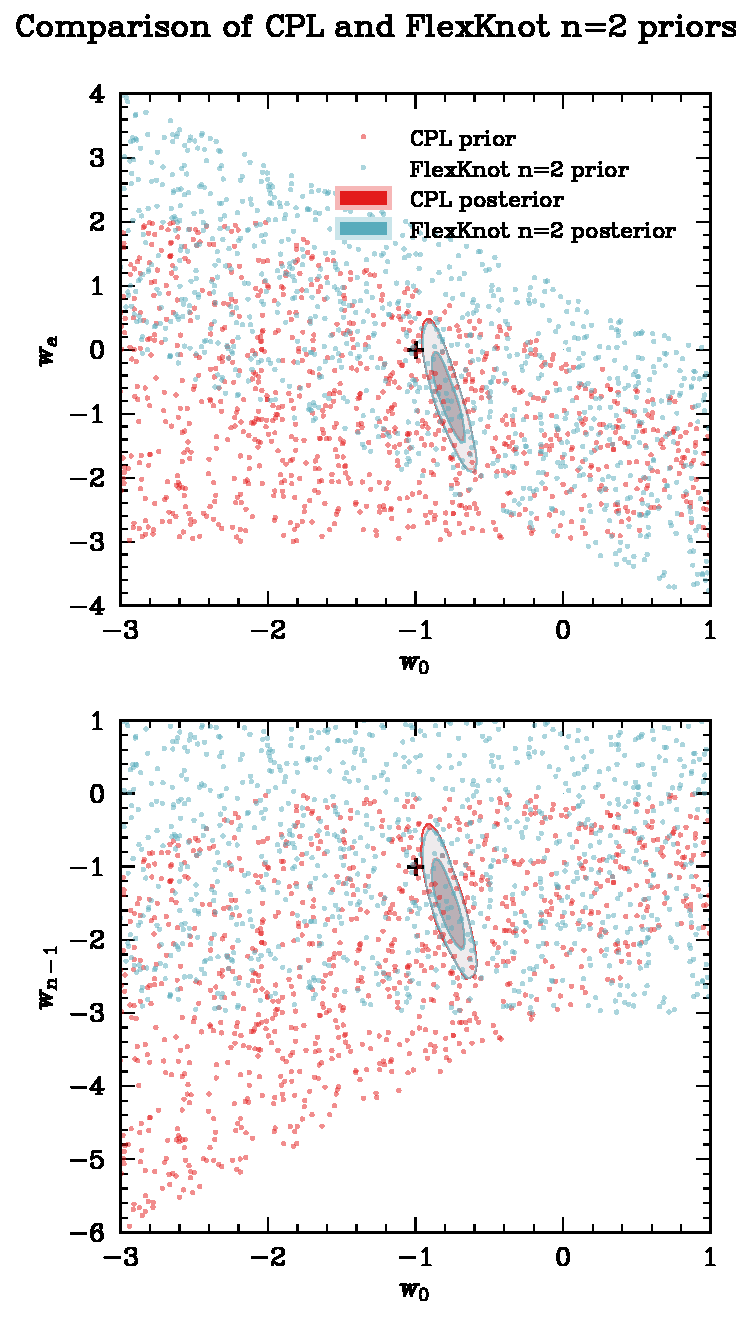
\includegraphics[width=0.48\textwidth]{plots/cplprior.pdf}
        \end{center}
        \caption{
            Prior and posterior of CPL and $n=2$ flexknot, using DES-5Y combined with DESI BAO.
            The top panel shows the $(w_0, w_a)$ projection, the lower panel shows $(w_0, w_{n-1})$.
            Prior samples are shown as a scatter, the posteriors are shown as kernel density estimates.
            For reference, the cross marks \lcdm{}.
            The two posteriors are so similar that it is challenging to see one on top of the other!
        }\label{fig:prior}
    \end{figure}

    \subsection{Nested bridge sampling}

    The nested sampling approach used previously and in this work computes the Bayesian evidence for each combination of data and model.
    However, in isolation, evidences are meaningless, and it is only with a pair that one can determine a Bayes factor, to which one may apply Jeffreys' scale \citep{jeffreys1939theory} to determine how to interpret the result, or combine with a model prior to determine the posterior odds.
    An alternative method to compute the Bayes factor, beside two normal nested sampling runs, is to use nested bridge sampling.

    Nested bridge sampling (NBS, \cite{chen2000monte, bridgetutorial}, Yallup et al. (in prep, due September $21^\text{st}$ 2025) makes use of the inevitable similarity between the posteriors for the shared parameters between sampling runs with nested models.
    This work consists entirely of nested models.
    \lcdm{} is nested within $w$CDM with $w=0$, which are both nested within CPL, which are all nested within flexknot models.
    Also, each cosmological model with $\dmb{}=0$ is nested within the same model with \dmb{} varying.
    In theory, one could bridge sample from vanilla \lcdm{} to an $n=20$ flexknot with \dmb{}.
    As a demonstration, let us outline nested bridge sampling to add \dmb{} only to an existing run.

    Yallup (in prep) explains this method in detail and its application to toy and cosmological examples; let us recap the methodology here:
    The recipe is as follows: first, produce a set of samples with $\dmb{}=0$.
    Then, sample the likelihood ratio, $\tilde{\mathcal L}$, using the posterior from the first run as part of an effective prior:
    %
    \begin{equation}
        \tilde{\mathcal L}=\frac{\mathcal L(D|\theta, \dmb{})}{\mathcal L(D|\theta, \dmb{}=0)}\text, \quad 
        \tilde\pi = \pi(\dmb{}|\theta)\frac{\pi(\theta)\mathcal L(\theta)}{Z_1}\text,
        \label{eq:ratio}
    \end{equation}
    %
    where $D$ is the data (DES-5Y alone or with DESI BAO), and $\theta$ are the appropriate other parameters for the cosmology in question.
    These arise from rearranging the Bayes factor:
    %
    \begin{equation} \label{eq:ratioratio}
        \begin{aligned}
            \frac{Z_2}{Z_1} &= \frac{\int\mathcal L(\theta, \dmb{})\pi(\theta, \dmb{})\mathrm d\theta\mathrm d(\dmb{})}{Z_1} \\
            &= \int\underbrace{\frac{\mathcal L(\theta, \dmb{})}{\mathcal L(\theta)}}_{\tilde{\mathcal L}}
            \underbrace{\pi(\dmb{}|\theta)\frac{\pi(\theta)\mathcal L(\theta)}{Z_1}}_{\tilde\pi} \mathrm d\theta\mathrm d(\dmb{}) \text,
        \end{aligned}
    \end{equation}
    %
    where the data $D$ is suppressed from the likelihood for clarity, and the probability product rule has been used to factorise the prior $\pi(\theta, \dmb{}) = \pi(\dmb{}|\theta)\pi(\theta)$.
    The word ``nested'' should not be confused with the same in nested sampling, which refers to the onion of likelihood contours.
    However, nested sampling may indeed be used to perform nested bridge sampling, but one may substitute Sequential Monte Carlo \citep{smc}, which is what is used here, for both the initial sampling run and bridging, abbreviated as SMC-NBS.
    A possible disadvantage of SMC compared to nested sampling is that it does not report an error bar, the error bars here are from ten repeats with different initial random seeds.

    \subsection{\textsc{JAX} reimplementation}

    In addition to the pipeline from previous work, the likelihoods have also been ported to \textsc{JAX}.
    This allows them to be sampled using \textsc{BlackJAX} nested slice sampling, which makes use of GPU parallelisation \citep{yallup2025nested, metha, cabezas2024blackjax}.
    In fact, the $n=2$ flexknot prior and posterior shown in Figure~\ref{fig:prior} is from the \textsc{PolyChord} pipeline, which uses \textsc{numpy} and \textsc{scipy} and 64-bit floating point precision, while the CPL result uses the \textsc{JAX} pipeline, with 32-bit floating point precision.
    Reimplementation in \textsc{JAX} posed some additional challenges, for example, the adaptive \textsc{QUADPACK} method used to compute the integral over $\frac{H_0}{H(z)}$ is not available in \textsc{JAX.SCIPY}, so trapezoidal integration was substituted.
    Also, it was found that the precision setting for the Mahalanobis distance matrix multiplication had to be increased from its default level for consistency with the other pipeline.
    Therefore, it is very reassuring that the results, which differ in hardware, sampler, 1-dimensional integration technique for proper motion distance, and floating point representation, are so similar.

    One feature of \textsc{PolyChord} currently omitted from the \textsc{BlackJAX} sampler is live point clustering.
    Clustering is typically considered necessary for nested sampling with multi-modal posteriors, however, the \textsc{BlackJAX} sampler has proven surprisingly effective on other problems.
    It is the subject of ongoing research whether no clustering is genuinely a limitation, therefore, we restrict the application of the \textsc{JAX} pipeline to the unimodal \lcdm{} and CPL likelihoods only in this work.

    \section{Results}\label{sec:results}

    \begin{figure}
        \begin{center}
            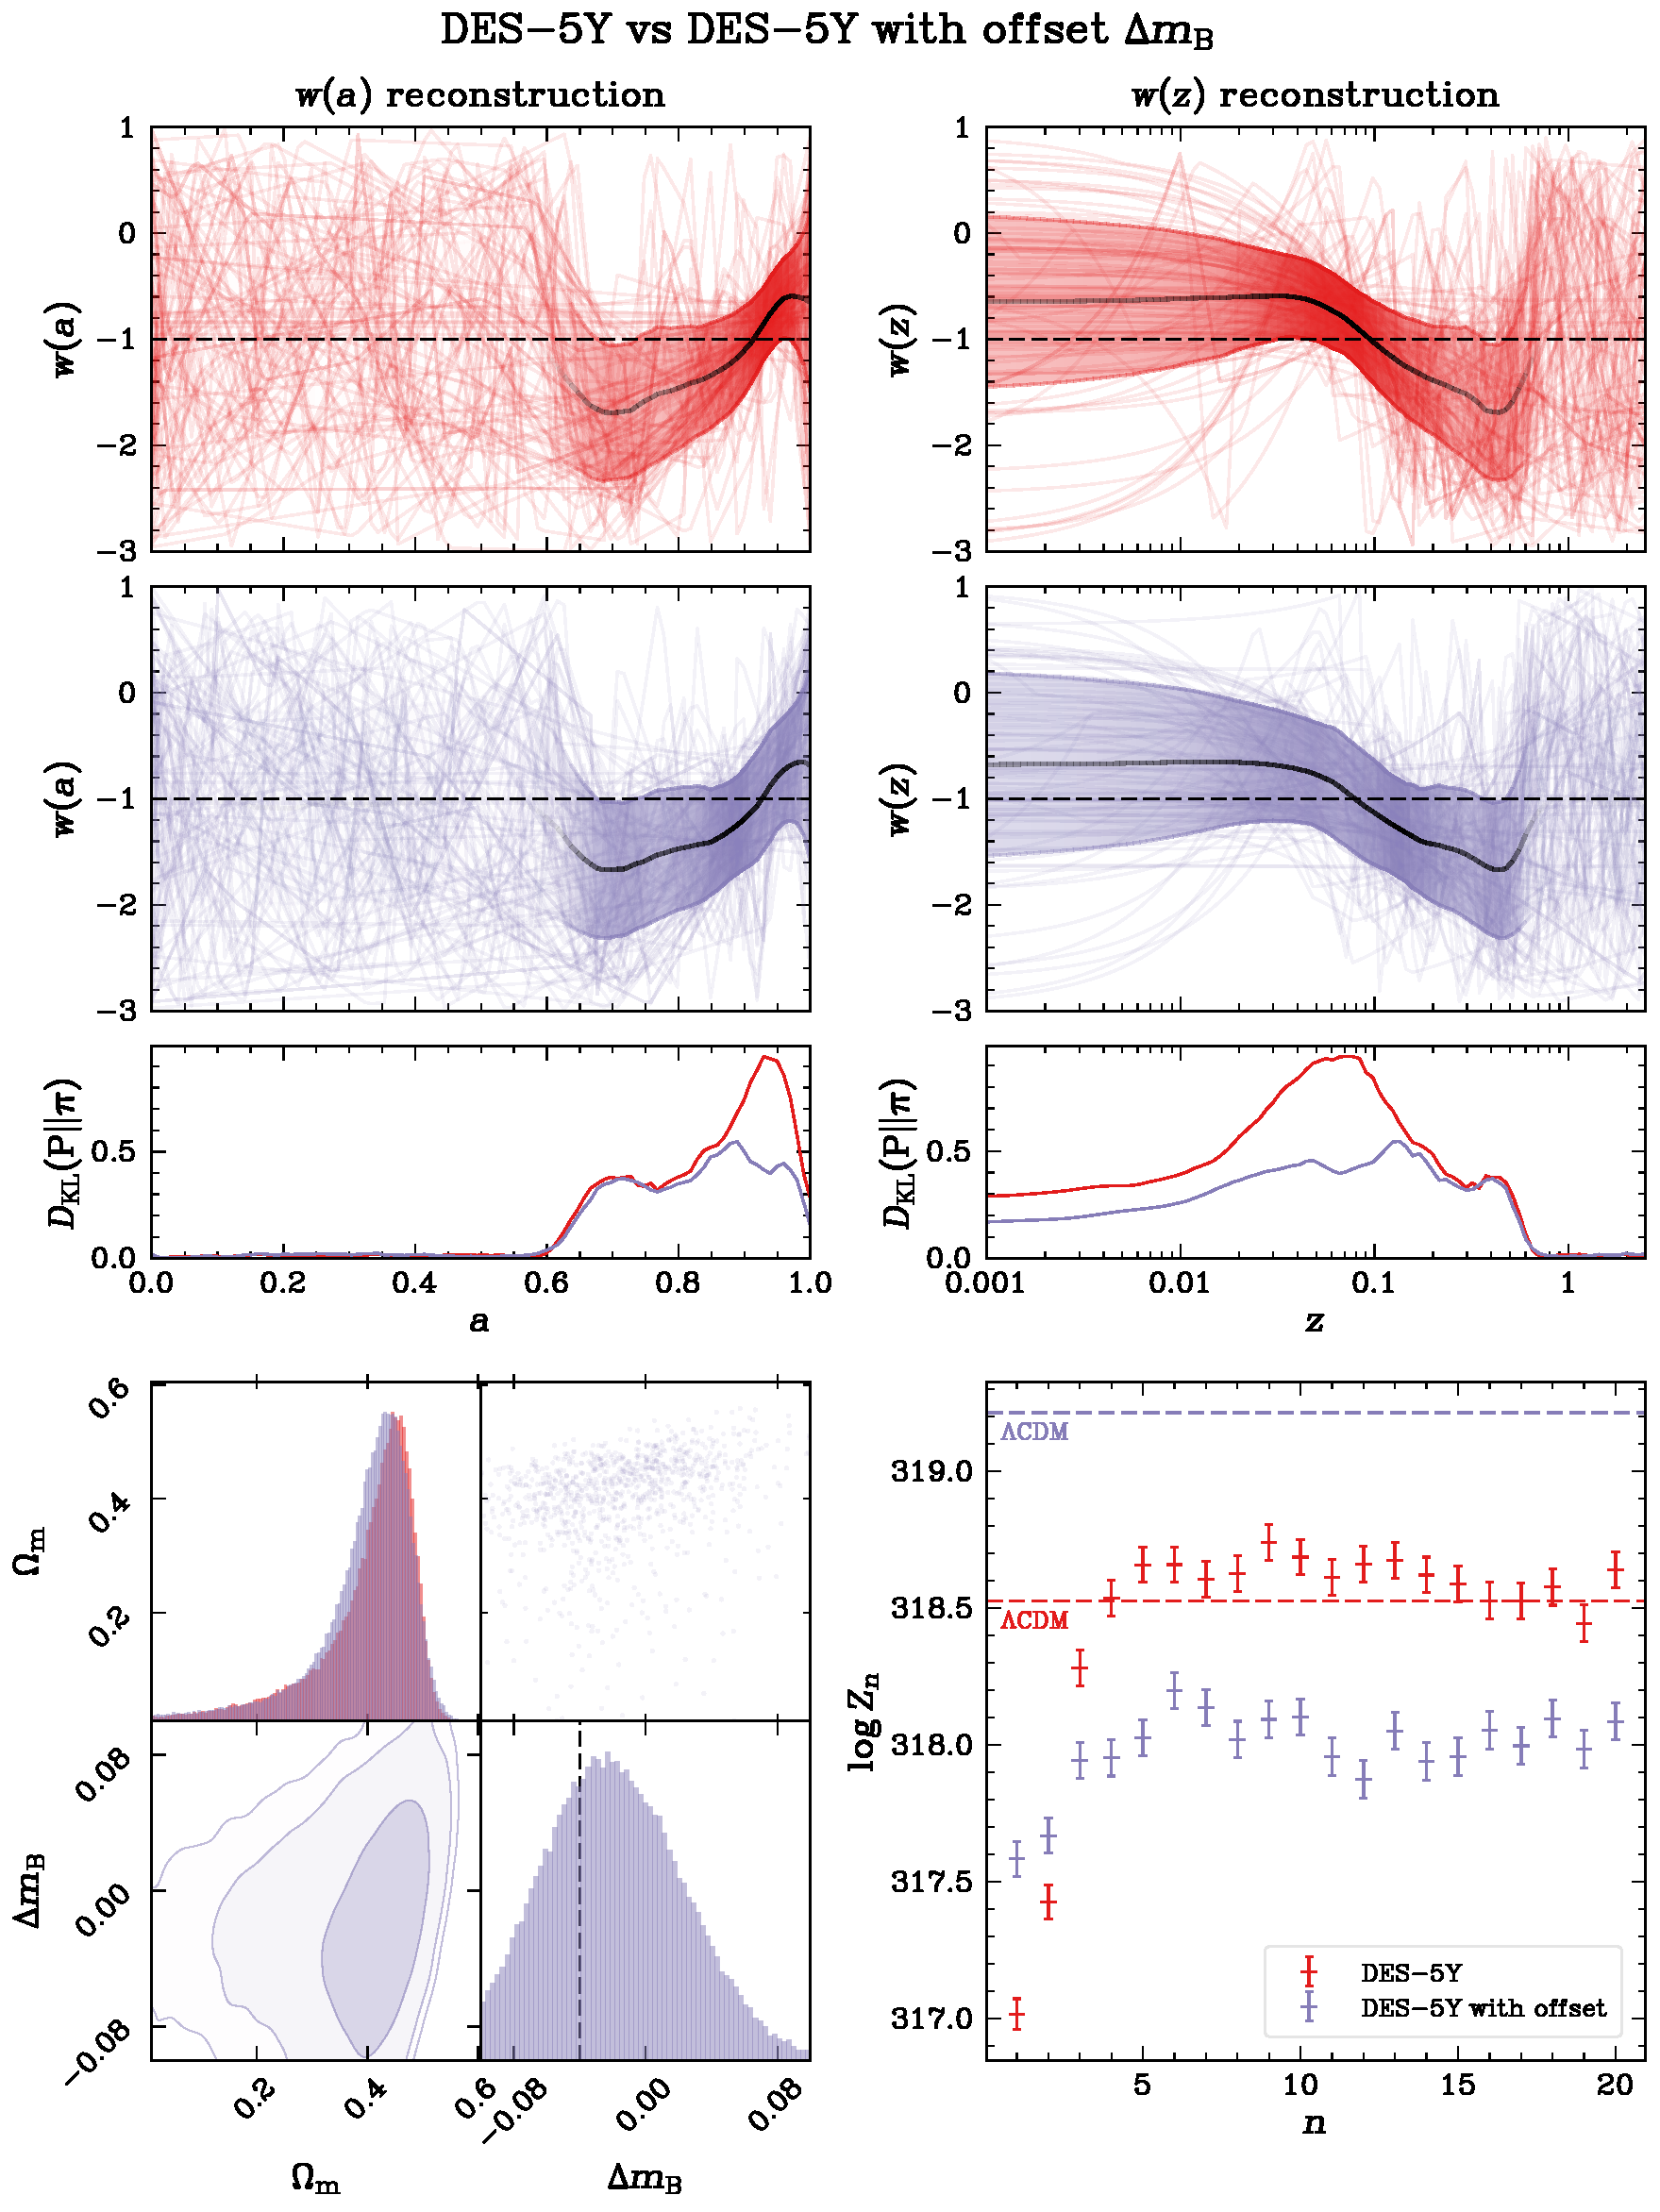
\includegraphics[width=0.48\textwidth]{plots/des5yoffset_20_wa.pdf}
        \end{center}
        \caption{
            Flexknot reconstruction of the dark energy equation of state parameter using DES-5Y supernovae only.
            In red is the standard likelihood, in lilac, the version with the \dmb{} offset for the low-redshift supernovae.
            The overall shape of the reconstructions are very similar, but the functional KL divergence and model evidences tell quite different stories.
            Firstly, note that the high-$a$/low-redshift KL divergence lacks the peak just below $z=0.1$, which is to be expected as allowing those magnitudes to float up and down will naturally reduce their constraining power.
            Second, note that the evidence for \lcdm{} has increased with the offset, meanwhile, it has fallen for all flexknots with more than three knots.
            The Bayes factor between \lcdm{} and $w$CDM is similar between the two likelihoods, but $n=2$ is more disfavoured with the offset likelihood.
            Crucially, the evidence for \lcdm{} with the offset is greater than the flexknots without the offset.
            This suggests that the complexity demanded by the flexknot model is just as well, if not better, met by including this additional degree of freedom.\\
            Please note that the posteriors shown in the bottom-left panels do not include \lcdm{}, which is shown separately in Figure~\ref{fig:dmb}.
            With flexknots, \dmb{} is not well constrained.
        }\label{fig:des5y}
    \end{figure}
    
    \begin{figure}
        \begin{center}
            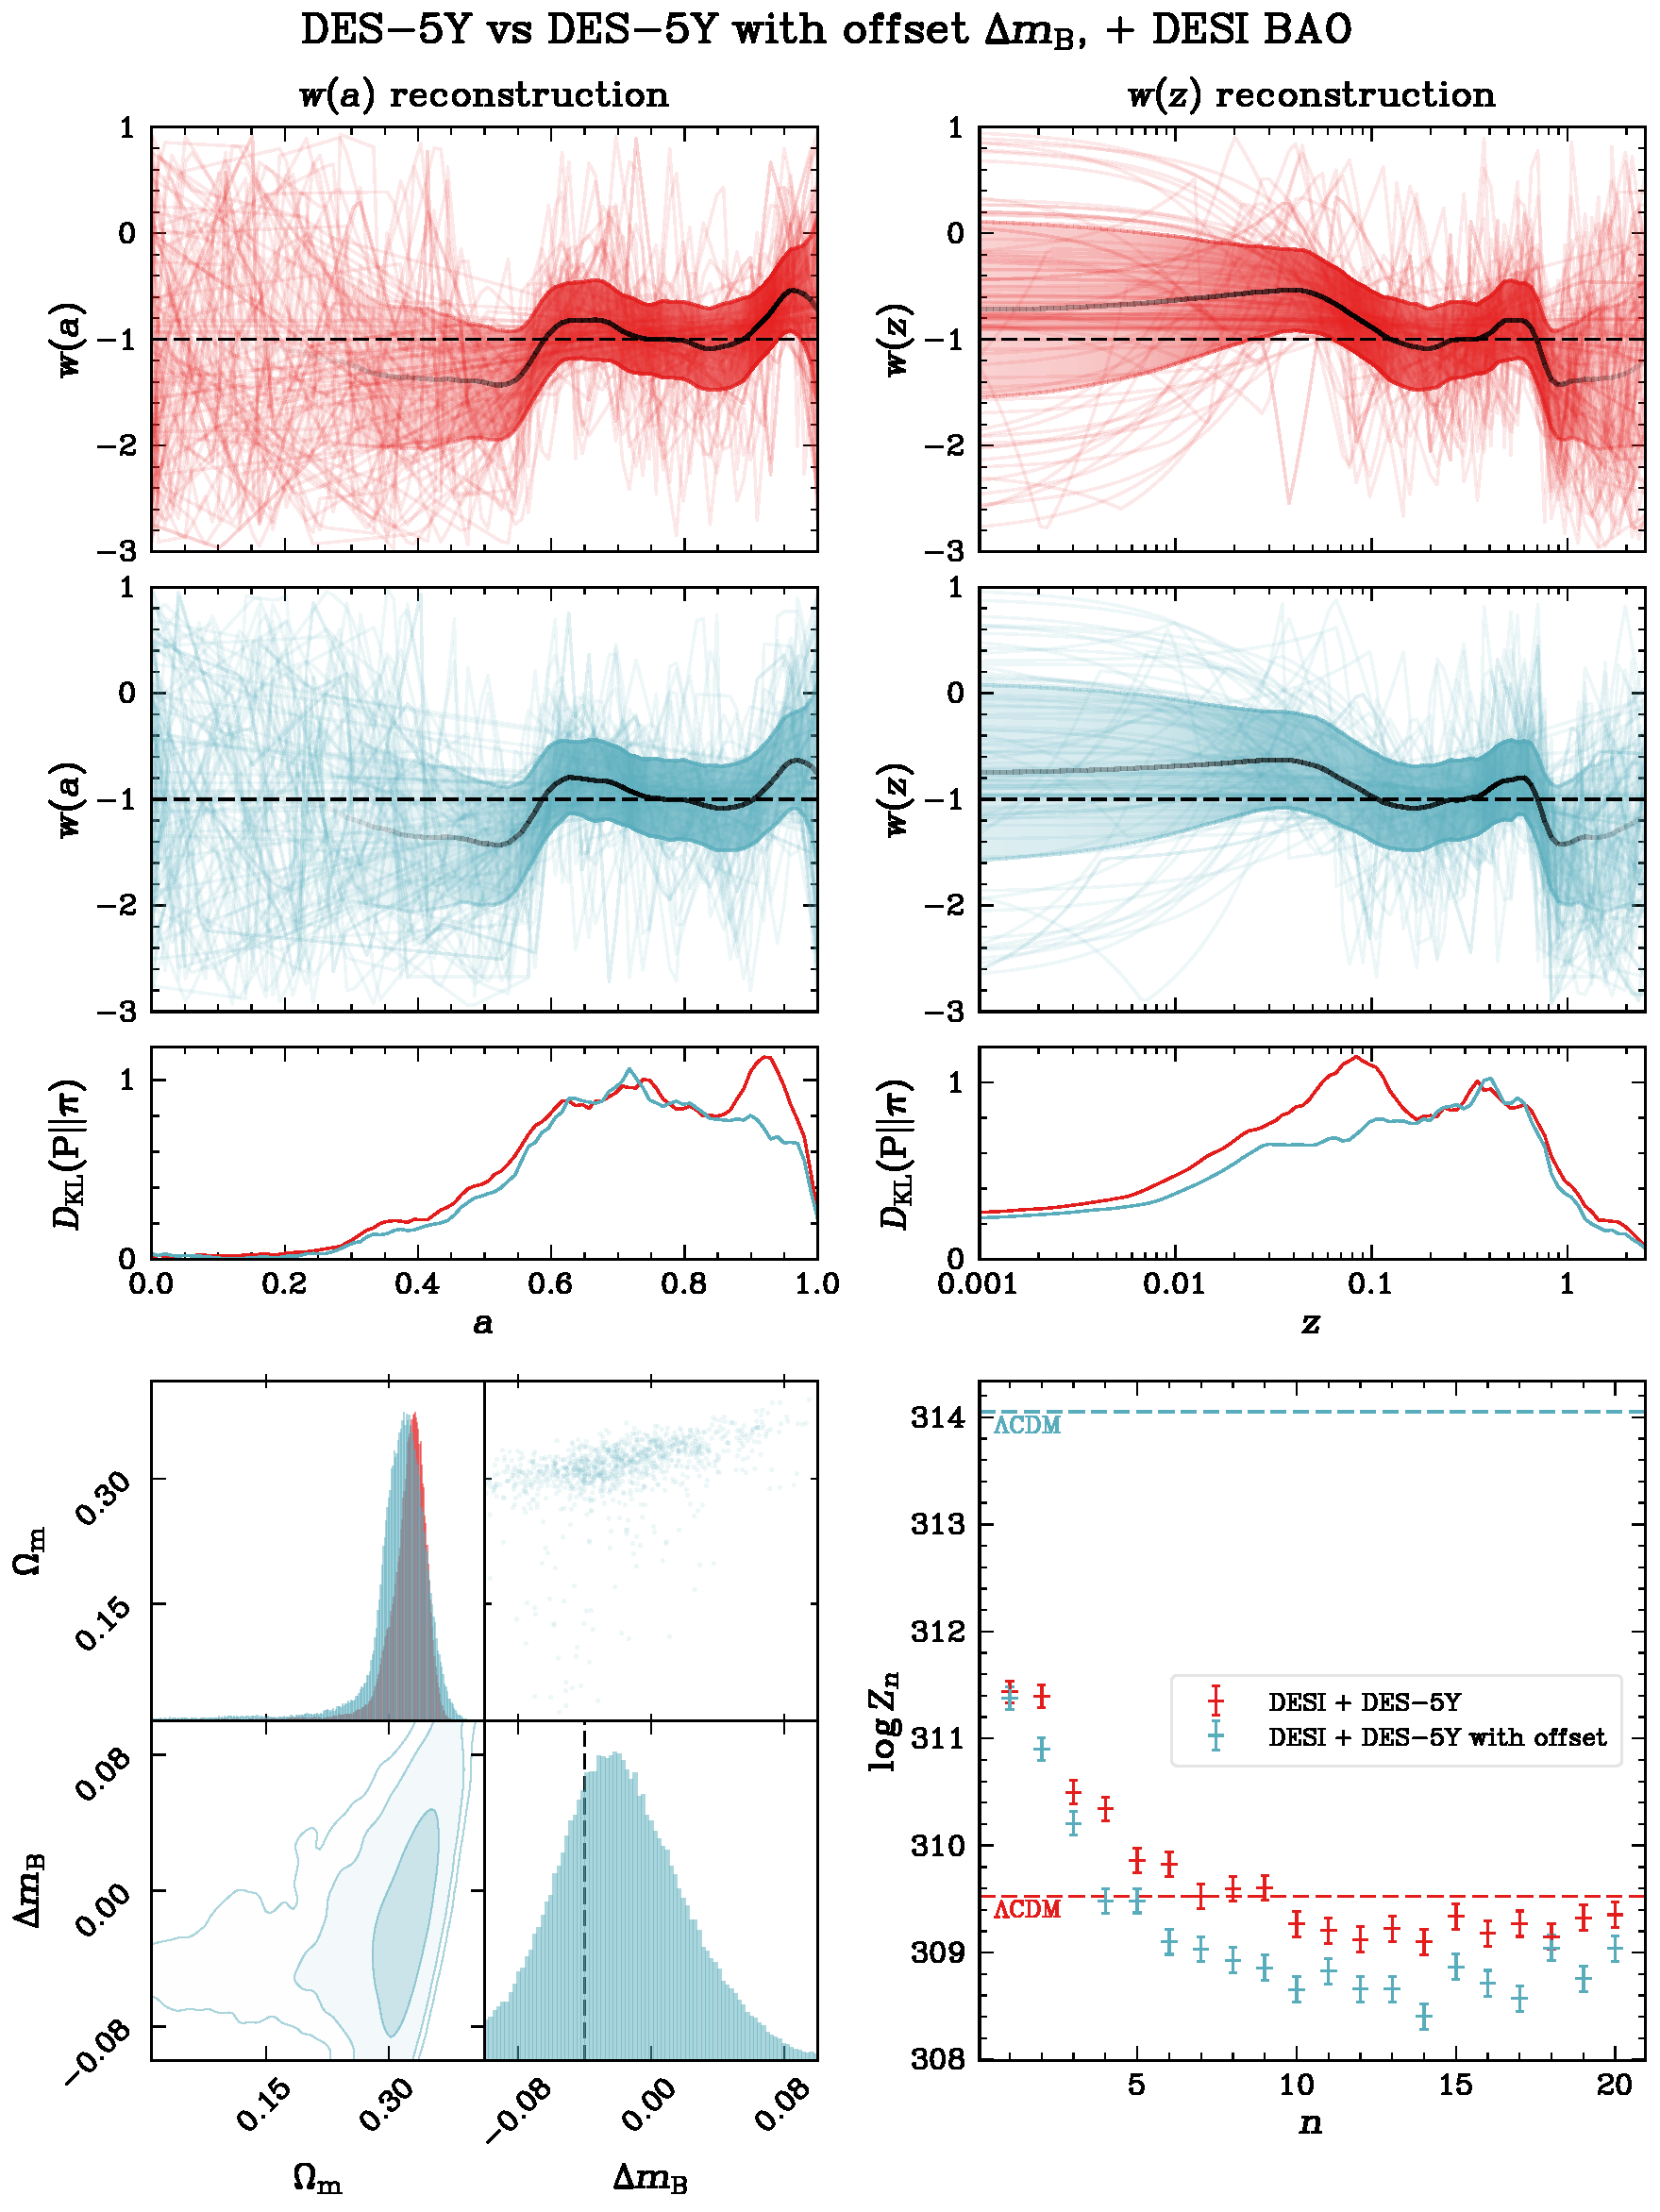
\includegraphics[width=0.48\textwidth]{plots/desidr2_des5yoffset_20_wa.pdf}
        \end{center}
        \caption{
            Similar to Figure~\ref{fig:des5y}, this time with the addition of DESI BAO.
            This time, it is even clearer that \lcdm{} with the \dmb{} offset is the favoured model.
            Once again, the low-redshift KL divergence peak is lost with the additional parameter.
            Unlike the results with DES-5Y alone, the Bayes factor for \lcdm{} with \dmb{} over almost any other model is ``decisive''.
            Again, please note that the posteriors shown in the bottom-left panels do not include \lcdm{}, these are shown in Figure~\ref{fig:dmb}.
        }\label{fig:desidr2des5y}
    \end{figure}

    \begin{figure}
        \begin{center}
            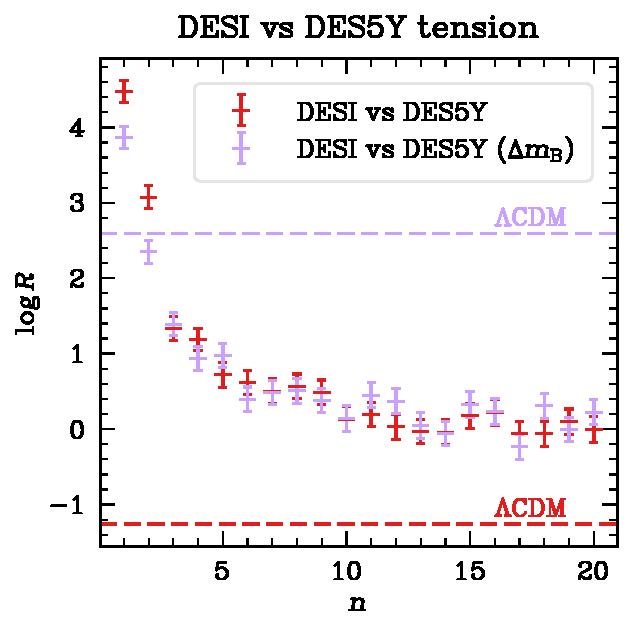
\includegraphics[width=0.4\textwidth]{plots/tension.pdf}
        \end{center}
        \caption{
            Tension values between DES-5Y and DESI BAO, with and without the low-redshift offset.
            \lcdm{} is shown as horizontal dashed lines, for easy comparison with the other points.
            For \lcdm{} the tension has been reduced (more positive) significantly, while for $w$CDM and CPL, it has increased slightly.
            \lcdm{} with the offset is now on-par with CPL, though $w$CDM remains the model with the best dataset concordance.
            In contrast, without the offset, \lcdm{} is the most discrepant model of all.
            For three knots and above, the tension is similar with or without the offset.
        }\label{fig:tension}
    \end{figure}

    \begin{figure}
        \begin{center}
            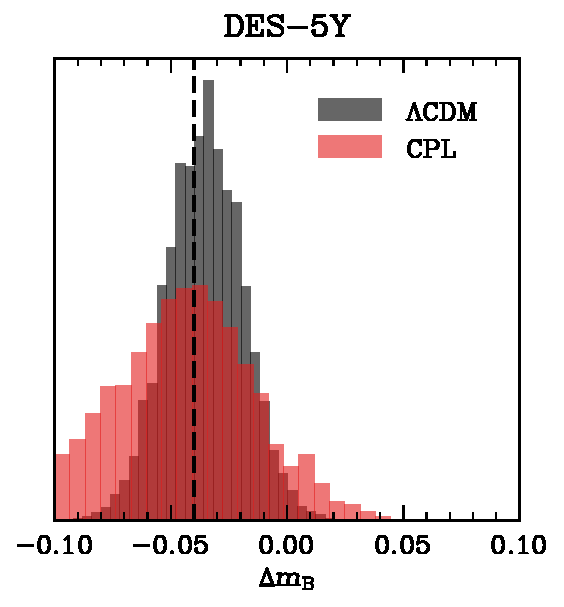
\includegraphics[width=0.23\textwidth]{plots/dmb_des5y.pdf}
            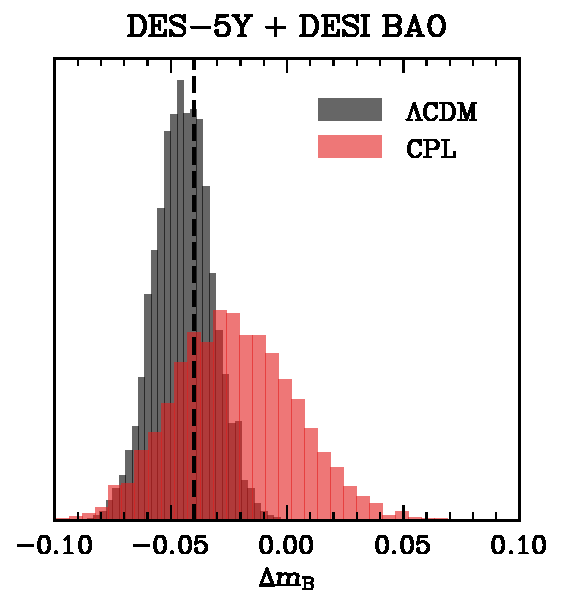
\includegraphics[width=0.23\textwidth]{plots/dmb_desidr2_des5y.pdf}
        \end{center}
        \caption{
            Posterior histograms of \dmb{} for \lcdm{} and CPL.
            The left panel uses DES-5Y only, the right also includes DESI BAO.
            The prior is uniform over the domain of the plot.
            As predicted by \citet{georgedes5y}, its value is centred on $-0.04$.
            Note that the \lcdm{} posteriors (and the right CPL posterior) are well contained within the prior, therefore, the evidence which would have been found had a wider prior been used can be easily be computed with the ratio of the prior volumes.
        }\label{fig:dmb}
    \end{figure}
    
    \begin{table}
        \caption{
            Values of \dmb{} for DES-5Y, along with the Bayes factor between the standard version ($\dmb{} = 0$) and with the offset.
            The Bayes factor is calculated in two ways, first by taking the ratio of the evidences from the nested sampling runs, and also by bridge sampling from $\dmb{}=0$ to the offset version.
            Bridge sampling is not attempted for the flexknot models, as more work is required to determine if this is viable.
            The shown nested sampling Bayes factors are from the \textsc{JAX} pipeline, which are consistent with the \textsc{PolyChord} pipeline, which are not reported here.\\
            Both \lcdm{} values of \dmb{} are consistent with $-0.04$, and inconsistent with zero to over $2\sigma$.
            In contrast, both CPL and flexknot dark energy do not exclude zero, this is reflected in the Bayes factors.
            Of particular note is the large positive Bayes factor for \lcdm{} with DES-5Y + DESI BAO in favour of a low-redshift supernova offset.
            The Bayes factors from SMC-NBS are beyond error of those computed from two nested sampling runs, but not so much to affect any conclusions.
        }\label{tab:des5y}
        \begin{center}
            \begin{tabular}[c]{|l|c|c|c|}
                \hline
                \multicolumn{4}{|c|}{DES-5Y}\\
                \hline
                & \dmb{} & Bayes factor & SMC-NBS \\
                \hline
                \lcdm{} & $-0.035 \pm 0.016$ & $0.755 \pm 0.098$ & $0.665 \pm 0.030$ \\
                CPL & $-0.042 \pm 0.028$ & $-0.067 \pm 0.127$ & $0.086 \pm 0.109$ \\
                flexknot & $-0.018 \pm 0.040$ & $-0.525 \pm 0.021$ & N/A \\
                \hline
                \multicolumn{4}{|c|}{DES-5Y + DESI BAO}\\
                \hline
                \lcdm{} & $-0.045 \pm 0.012$ & $4.140 \pm 0.182$ & $4.488 \pm 0.037$ \\
                CPL & $-0.022 \pm 0.026$ & $-0.859 \pm 0.217$ & $-0.738 \pm 0.018$ \\
                flexknot & $-0.017 \pm 0.038$ & $-0.396 \pm 0.055$ & N/A \\
                \hline
            \end{tabular}
        \end{center}
    \end{table}

    \subsection{Flexknot reconstructions}
    We begin with DES-5Y supernovae alone.
    Figure~\ref{fig:des5y} shows the flexknot reconstruction of $w(a)$ both with and without the low-redshift offset.
    From the KL divergence panels, it can be seen that the constraining power at low redshifts is reduced with the additional parameter; this is to be expected.
    The model with the greatest evidence is \lcdm{} with the offset.
    This suggests that the complexity picked up by the flexknot model, which brings models with four or more knots in line with \lcdm{}, is better explained by \dmb{}.
    Only \lcdm{}, $w$CDM and CPL ($n=1$ and $n=2$ respectively) have greater evidence with the introduction of the offset; the reverse is true for three or more knots.
    However, at least with DES-5Y alone, these suggestions must be caveated by the relatively small Bayes factors between evidences with the same $n$, which are at most around $0.7$.
    In fact, Jeffreys' scale suggests that these differences are ``barely worth mentioning''.
    We will return to this in Section~\ref{sec:priorwidth}.

    When the DESI data are included, the combined reconstruction is shown in Figure~\ref{fig:desidr2des5y}.
    With the BAOs, \lcdm{} with \dmb{} is still the favoured model, this time, with a log-Bayes factor of around four over almost all other models, crucially including standard \lcdm{}.
    The offset has also removed the preference for low numbers of flexknots.
    This strongly suggests that the original preference for dynamical dark energy can be better accounted for by this offset than it can by $w$CDM, CPL, or even flexknots.

    The \textsc{JAX} pipeline produced \lcdm{} and CPL evidences in perfect agreement with those from \textsc{PolyChord}; in fact, it is those reported in Table~\ref{tab:des5y}.
    These nested sampling runs completed in less than a second on a Google Compute Engine Nvidia L4 GPU, plus a few seconds of compile time.
    This compares very well to tens of minutes on a 76-core CSD3 CPU, plus submission delay, and has the potential to transform the typical Bayesian's workflow.

    It is important to assess how \dmb{} may affect the possibility of tension between DES-5Y and DESI BAO.
    Once again, we follow \cite{paper1}, using the techniques developed in \cite{lemos, hergt, balancingact} via the $\log R$ statistic.
    The results are shown in Figure~\ref{fig:tension}.
    Without the offset, \lcdm{} is the most discrepant model, with the only negative $\log R$.
    With the offset, \lcdm{} is now on par with CPL, while $w$CDM remains the model with the best concordance between the two datasets.
    For three knots and above, the tension is similar with or without the offset.
    This is reassuring, as it suggests that the offset is better able to explain the discrepancy between the datasets than flexknot dark energy.

    \subsection{Effect of \dmb{} prior width}\label{sec:priorwidth}
    
    From Figure~\ref{fig:dmb}, it can be seen that, for \lcdm{}, the posterior for \dmb{} is reasonably well contained within our chosen prior.
    This allows us to examine the Bayes factors in more detail.

    The uniform prior contains a factor of the reciprocal of the prior volume $V$, which, in the well contained case, persists into the Bayesian evidence.
    This means that the evidence that \textit{would} have been found for a different, wider, uniform prior can be calculated as:
    %
    \begin{equation}
        \log Z \rightarrow \log\left(Z\times\frac{V_\text{narrow}}{V_\text{wide}}\right) = \log Z - \log\frac{V_\text{wide}}{V_\text{narrow}}\text.
        \label{eq:}
    \end{equation}
    %
    Our prior of $\dmb\in[-0.1, 0.1]$ was chosen to be relatively narrow for two reasons: firstly, the nested sampling runtime is proportional to the KL divergence from prior to posterior; second, if the low-redshift systematic offset does exist and had a value beyond this range, it is unlikely that it would fall to third parties to investigate it, and frankly this should impact on our model prior.
    For example, let us examine our conclusions if a prior ten times wider, $[-1.0, 1.0]$, had been chosen.
    This would reduce Bayes factors by approximately $\log 10 = 2.30$.
    Consider DES-5Y alone: the only positive Bayes factor is \lcdm{} at around $0.76$, this would be reversed with this more liberal prior.
    In fact, we may reverse-engineer this argument to note that, had a prior $e^{0.76}\approx2.14$ times larger been chosen, the Bayes factor would have been precisely zero.
    One may rightly criticise that post-hoc revisions to the prior are unwise, however, if this were all the data we had, it seems this would be enough to suggest that there is no practical evidence for the low-redshift offset, since it is so vulnerable to somewhat reasonable alternative priors.

    However, now reintroduce the DESI BAO, with a Bayes factor of $\log Z = 4.140\pm0.127$ in favour of \dmb{}.
    This time, one would have needed a prior at least sixty-two times wider to reverse the conclusion --- an offset of such magnitude is completely unreasonable.
    Therefore, we will conclude that there is only evidence for the low-redshift supernova offset in DES-5Y if, and only if, it is combined with baryon acoustic oscillations, and \lcdm{} is correct.

    \subsection{Nested bridge sampling Bayes factors}

    Table~\ref{tab:des5y} also includes the SMC-NBS Bayes factors.
    Error bars were estimated by running SMC-NBS ten times with different random seeds, while those from nested sampling were computed using \textsc{anesthetic}, which samples possible nested sampling volume compression histories \citep{anesthetic}.
    It is interesting that all four of the NBS error bars are tighter than those from nested sampling.
    The different approaches, in some cases, like outside the error of each other, though not so significantly as to affect any conclusions.
    For example, it is not surprising that the very small Bayes factors with CPL DES-5Y have the opposite signs.
    Crucially, the Bayes factor of the most interest, which happens to be the largest, of \dmb{} or no \dmb{} with DESI in \lcdm, is similarly large with NBS.
    The SMC implementation also uses \textsc{BlackJAX}, and similarly takes mere seconds to run.
    
    \section{Conclusions}\label{sec:conclusions}

    In this work, it has been found that there is substantial Bayesian evidence for a low-redshift supernovae systematic in DES-5Y, when it is combined with DESI BAO.
    However, without the BAO, the claim is unsubstantiated, though the posterior on the offset value indeed agrees with the $-0.04$ of \citet{georgedes5y} and excludes zero to $2\sigma$.
    Crucially, the Bayesian evidence favours offset \lcdm{} over flexknot dark energy with or even without the offset, so we must conclude that the systematic is a better model than dynamical dark energy.
    We accept that this approach is limited, and adjusting a subset of apparent magnitudes post bias correction does not constitute a sensible supernova catalogue.
    Nevertheless, the options are clear: either there is a systematic issue with the DES-5Y supernovae, or dark energy really is dynamical.

    It has also been found that the \lcdm{} tension between DES-5Y and DESI BAO is significantly reduced with \dmb{}, while $w$CDM and CPL tensions are slightly increased.
    $w$CDM still remains the model with the best agreement.

    The alternative \textsc{JAX} pipeline has produced \lcdm{} and CPL posterior samples and evidences in excellent agreement with those from our original \textsc{PolyChord}-powered approach.
    The reduced sampling time to mere seconds has the potential to be transformative for the Bayesian workflow.
    We leave it for future work to investigate whether these tools are robust for the more challenging multi-modal posterior of flexknot reconstructions.
    We also find that Bayes factors obtained using nested bridge sampling are sufficiently similar to those obtained by the ratio of nested sampling evidences. Therefore, we hope that this approach can be trialled more widely.

    \section*{Acknowledgements}

    A.N.~Ormondroyd and W.J.~Handley were supported by the research environment and infrastructure of the Handley Lab at the University of Cambridge.
    This work was performed using the Cambridge Service for Data Driven Discovery (CSD3), part of which is operated by the University of Cambridge Research Computing on behalf of the STFC DiRAC HPC Facility (\url{www.dirac.ac.uk}).
    The DiRAC component of CSD3 was funded by BEIS capital funding via STFC capital grants ST/P002307/1 and ST/R002452/1 and STFC operations grant ST/R00689X/1.
    DiRAC is part of the National e-Infrastructure.
    WJH was supported by a Royal Society University Research Fellowship.
    The authors thank David Yallup and Toby Lovick for guidance with SMC-NBS.

    %%%%%%%%%%%%%%%%%%%%%%%%%%%%%%%%%%%%%%%%%%%%%%%%%%
    \section*{Software and Data Availability}

    The \textsc{python} pipeline in this work made use of \textsc{NumPy} \citep{numpy}, \textsc{SciPy} \citep{scipy}, and \textsc{pandas} \citep{pandaszenodo, pandaspaper}.
    The GPU-accelerated pipeline was written in \textsc{JAX} \citep{jax2018github}, and supported by the Google Cloud research credits program, with the award GCP397499138.
    The nested sampling chains were analysed using \textsc{anesthetic} \citep{anesthetic}; plots were produced in \textsc{matplotlib} \citep{matplotlib}, using the \textsc{smplotlib} template created by \citet{smplotlib}.
    The \textsc{Python} and \textsc{JAX} pipelines and nested sampling chains used in this work can be obtained from Zenodo \citep{ormondroyd_2025_15025604}.

    %%%%%%%%%%%%%%%%%%%% REFERENCES %%%%%%%%%%%%%%%%%%

    % The best way to enter references is to use BibTeX:

    \bibliographystyle{mnras}
    \bibliography{desi3} % if your bibtex file is called example.bib

    % Alternatively you could enter them by hand, like this:
    % This method is tedious and prone to error if you have lots of references
    %\begin{thebibliography}{99}
    %\bibitem[\protect\citeauthoryear{Author}{2012}]{Author2012}
    %Author A.~N., 2013, Journal of Improbable Astronomy, 1, 1
    %\bibitem[\protect\citeauthoryear{Others}{2013}]{Others2013}
    %Others S., 2012, Journal of Interesting Stuff, 17, 198
    %\end{thebibliography}

    %%%%%%%%%%%%%%%%%%%%%%%%%%%%%%%%%%%%%%%%%%%%%%%%%%

    %%%%%%%%%%%%%%%%% APPENDICES %%%%%%%%%%%%%%%%%%%%%


    \appendix

    \section{Analytic marginalisation over \dmb{}}\label{apx:marginalisation}

    This appendix contains an extension to the analytical marginalisation in \cite{paper1} and \cite{paper2}.
    In those works, it was demonstrated that the constant offset from $M_\mathrm B$ could be analytically marginalised from the SNe likelihoods.
    Since this value affects all terms in the data vector, there is essentially an accompanying mask of all ones.
    In fact, the algebra is identical for any mask, assuming that the likelihood tends to zero at the limits of the prior, so \dmb{} could be marginalised over by replacing the covariance matrix:
    %
    \begin{equation}
        \Sigma^{-1} \rightarrow \Sigma^{-1} - \frac{\Sigma^{-1} \mathbfit s^T\mathbfit s\Sigma^{-1}}{\mathbfit s^T\Sigma^{-1}\mathbfit s} \text,
    \end{equation}
    %
    and adjusting the normalisation by a factor of $\frac 1 {V_\mathbfit s}\sqrt{\frac{2\pi}{\mathbfit s^T\Sigma\mathbfit s}}$, where $V_\mathbfit s$ is the prior volume of the offset, \dmb{} in this case.
    However, this introduces two challenges.
    First, each one of these marginalisations introduces an additional zero eigenvalue to the inverse covariance matrix, reducing its rank by one.
    This introduces precision issues, in particular when working in 32-bit floating point.
    Secondly, the posterior of \dmb{} is of interest, and while it is possible to then sample it from the posterior of the other parameters, it is more straightforward to simply include it as a parameter during nested sampling, as this poses no challenge for our nested slice sampling tools.

    \section{Effect of CPL prior on evidence and tension}\label{apx:prior}

    This appendix investigates the impact of the difference between the flexknot and CPL priors on their Bayesian evidences and the tension ratio.
    The Bayesian evidence may be split into two terms, the average log-likelihood over the posterior, and the KL divergence from prior to posterior:
    %
    \begin{equation}
        \log Z = \langle\log\mathcal L\rangle_\mathcal P - \mathcal D_\mathrm{KL}(\mathcal P||\pi)\text.
    \end{equation}
    %
    In the uniform prior case, the KL divergence may be further simplified to:
    %
    \begin{equation}
        \begin{aligned}
            \mathcal D_\mathrm{KL}(\mathcal P||\pi) &= \int \mathcal P(\theta)\log\frac{\mathcal P(\theta)}{\pi(\theta)}\mathrm d\theta\\
            &= \int\mathcal P(\theta)\log\mathcal P(\theta)\mathrm d\theta - \int\mathcal P(\theta)\log\pi(\theta)\mathrm d\theta\\
            &= \int\mathcal P(\theta)\log\mathcal P(\theta)\mathrm d\theta + \log V_\pi\text,
        \end{aligned}
    \end{equation}
    %
    where $V_\pi$ is the prior volume.
    Assume that the two posteriors are very similar, as is the case for CPL and $n=2$ flexknots, then the posterior-averaged log-likelihoods will be approximately equal.
    From Table~\ref{tab:priors}, the flexknot prior volume is 16, while the CPL prior volume is 15.5.
    Therefore, the CPL log-evidences are expected to be $\log\frac{16}{15.5}\approx0.03$ greater than those for $n=2$ flexknots.

    Consider the expression for the tension ratio:
    %
    \begin{equation}
            \log R = \log Z_\mathrm{SNe+BAO} - \log Z_\mathrm{SNe} - \log Z_\mathrm{BAO}\text.
    \end{equation}
    %
    It can be seen that the tension ratio for CPL is expected to be approximately $0.03$ less than the equivalent flexknot.
    This difference is not negligible, but small compared to the sampling uncertainty in the evidences themselves, see Table~\ref{tab:des5y} and Figure~\ref{fig:tension} for examples.

    %%%%%%%%%%%%%%%%%%%%%%%%%%%%%%%%%%%%%%%%%%%%%%%%%%


    % Don't change these lines
    \bsp	% typesetting comment
    \label{lastpage}
\end{document}

% End of mnras_template.tex
